\chapter{ESPECIFICAÇÃO DO PROJETO} % (fold)
\label{cha:especificacao_do_projeto}

% Retirar web semântica e redefinir o projeto como o desenvolvimento de um sistema de recomendação com base em confiança acoplado a uma rede social.

 O projeto consiste no desenvolvimento de um sistema de recomendação acoplado a redes sociais e compatível com padrões utilizados na web semântica.

\section{Visão Geral do Sistema} % (fold)
\label{sec:visao_do_sistema}
 Os principais blocos do sistemas podem ser vistos na Figura~\ref{fig:escopo}.

\begin{figure}
  \centering
  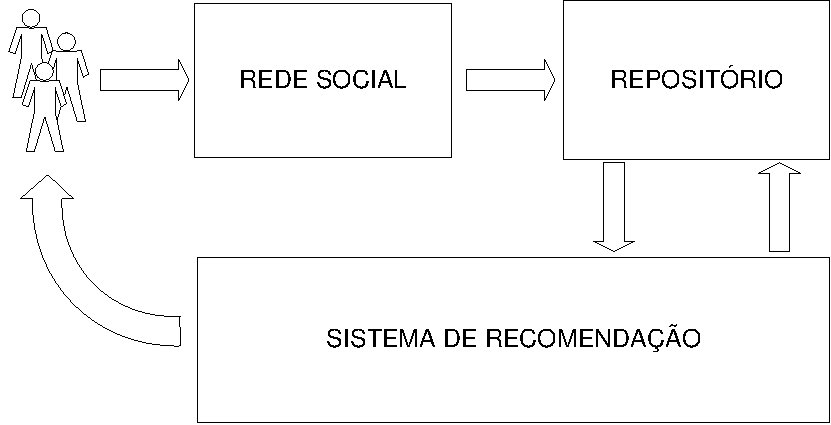
\includegraphics[width=\textwidth]{imagens/Diagrama_Visao_Geral}
  \caption{\it Diagrama de blocos do sistema}
  \label{fig:escopo}
\end{figure}

% Arrumar o laço de amizade, um usuário não faz um pedido a outro para ser amigo

 O sistema de recomendação utilizará redes sociais para obter as informações pessoais e as relações de amizade entre usuários. Neste contexto, um usuário é considerado amigo de outro quando eles estabelecem uma conexão direta dentro da rede social por meio de pedido de um usuário a outro, utilizando uma ferramenta própria do sistema.

% Retirar informação da confiança explícita

 Os usuários podem receber as recomendações dos seus amigos, ou de outras pessoas presentes na rede social. No entanto, as recomendações feitas por amigos serão consideradas, a princípio, mais importantes do que as realizadas por desconhecidos. Além da amizade, haverá uma relação explícita de confiança que será utilizada para determinar maior relevância da recomendação. Quando a relação de amizade no sistema é estabelecida, os dois usuários envolvidos devem escolher uma opção indicando o quanto eles confiam na pessoa que se tornará sua amiga para realizar boas recomendações de produtos.

% Retirar parágrafo

 O sistema de recomendação obtém informações a partir de documentos semanticamente estruturados que descrevem as avaliações dos produtos, as relações de amizades e as informações básicas dos usuários. Um repositório será implementado para armazenar tais informações, porém qualquer fonte de documentos que utilizem os padrões definidos pelo sistema de recomendação poderá ser utilizada. Desta forma, o sistema se integra ao contexto da web semântica.


% section visao_do_sistema (end)

\section{Descrição do Sistema}

% Retirar informação de cadastro de produtos

 Através do sistema os usuários poderão cadastrar produtos e avaliá-los quantitativamente, sendo possível realizar recomendações a outros usuários. Estes irão fornecer um feedback de tais recomendações, atualizando o valor da reputação do usuário que a forneceu. O sistema de recomendação filtra as informações recebidas por todos os usuários, de modo que apenas aquelas relevantes cheguem ao conhecimento das pessoas. As recomendações geradas pelo sistema são baseadas nas opiniões, nas relações sociais entre os usuários e nas relações encontradas entre os produtos e é o sistema que determina, a partir desses valores, o quão relevante é a recomendação realizada de um usuário para outro. Com base na relação entre usuários, produtos e avaliações o sistema irá inferir as seguintes informações:
 
\begin{itemize}

 \item Similaridade entre usuários

 \item Similaridade entre produtos

 \item Grau de confiança nas recomendações de um usuário para outro

 \item Grau de reputação global de um usuário baseado nas recomendações diretas

 \item Relação de consumo entre diferentes produtos

 \item Recomendações de produtos mais relevantes para um determinado usuário

\end{itemize}

 Para a obtenção das recomendações será feito um estudo para determinar quais critérios inferidos são mais importantes de forma que o sistema apresente uma boa acurácia, abrangência e alta satisfação dos usuários.

% Retirar informação de cadastro de produto

 Ao entrar na rede, o usuário tem a opção de buscar produtos já cadastrados e, caso não existam, cadastrá-los. Neste cadastro, ele pode informar a sua opinião referente ao produto e avaliá-lo, possibilitando ao sistema verificar quais são os seus interesses. Com isso, as pessoas podem recomendar os produtos para seus amigos presentes na rede social, sendo que esta deve ser direcionada para as pessoas que o usuário tenha certo conhecimento que gostarão do produto.

% Explicar melhor a relação de confiança entre usuários

 Os usuários que recebem a recomendação podem acessar o cadastro do produto e avaliá-lo para que o sistema atualize as informações relativas aos seus interesses. Estas informações são utilizadas para verificar a similaridade entre usuários. A avaliação altera o grau de reputação entre o usuário que recomendou o produto e o que recebeu. Caso a avaliação tenha um grau positivo, a reputação do receptor aumenta, porém, caso a avaliação tenha um grau negativo, significa que o usuário que recebeu a recomendação não a aceitou como relevante, fazendo com que o grau de reputação no outro usuário diminua.

 O sistema armazena todas essas informações referentes às avaliações de produtos, confiança e reputação entre usuários para filtrar recomendações entre usuários com baixo grau de confiança. Esse é um dos propósitos do sistema de recomendação: mostrar ao usuário apenas informações relevantes. Assim, caso a pessoa receba recomendações sem conteúdo plausível de um usuário, seu grau de reputação diminui e, quando esta diminuir até um limite, o sistema passa a não mostrar mais recomendações dele em destaque, sendo estas mostradas apenas como uma espécie de spam, mas ainda acessíveis ao usuário que as recebe.

 Também é função do sistema de recomendação realizar recomendações aos usuários para incentivar a avaliação de produtos, pois é assim que as pessoas fornecem informações referentes aos seus interesses. Tais recomendações são relativas aos produtos mais bem avaliados na rede e também aqueles bem avaliados por amigos com alto grau de reputação.

\section{Funcionalidades principais} % (fold)
\label{sec:funcionalidades_principais}

Abaixo estão sumarizadas as principais funcionalidades do sistema acompanhadas das descrições em formato de \textit{user stories}:
% referencia faltando!!!

\begin{itemize}

	\item Recomendação de produtos baseada em preferência do usuário
	\subitem Como usuário, eu quero receber uma lista de produtos que eu provavelemente goste para que eu não precise filtrar os itens que me interessam.

	\item Permitir que o usuário avalie um produto
  \subitem Como usuário, quero fazer a minha avaliação de produtos para que outros tenham conhecimento da minha opinião.

	\item Permitir que o usuário envie uma recomendação a outro usuário
  \subitem Como recomendador, quero enviar uma recomendação de produto para outra pessoa para que ela conheça a minha opinião sobre este item.

% Retirar funcionalidade

	\item Exposição das avaliações em formatos abertos
  \subitem Como agente web, quero obter as avaliações dos usuários em formato padronizado (e aberto) para que possa interpretar estas avaliações.

% Retirar funcionalidade

    \item Cadastro de novos produtos
    \subitem Como usuário, quero poder cadastrar um novo produto que ainda não está cadastrado.
    
% Retirar funcionalidade

    \item Importação de conteúdo em formato aberto
    \subitem Como usuário, quero poder informar uma fonte de conteúdo em formato aberto para que possa adicionar dados externos ao repositório.

    \item Explicação da recomendação
    \subitem Como usuário, quero obter a explicação sobre as recomendações recebidas para analisar criticamente a recomendação e me motivar a avaliar o produto.

    \item Visualização das avaliações recentes dos amigos
    \subitem Como usuário, quero estar ciente sobre as últimas avaliações dos meus amigos para que eu possa saber o que acontece no meu contexto social e conheça novos produtos.

    \item Feedback de recomendação
    \subitem Como recomendador, quero receber feedback sobre as recomendações que enviei para me incentivar a fazer melhores recomendações.

	
\end{itemize}

\section{Requisitos não-funcionais}

Os principais requisitos não-funcionais do sistema são:

\begin{itemize}

    \item Interface web compatível as últimas versões dos \textit{browsers} Internet Explorer, Mozilla Firefox e Safari.
    
    \item \textit{Backend} compatível com servidores Linux.

    \item Tempo médio de resposta menor que 2 segundos para 10 usuários simultâneos quando executado em um servidor com processador Intel Core 2 Duo T7250 ou superior e 2 GB de memória RAM. % esta é a configuração do meu notebook -- Allan

\end{itemize}

\section{Limites do Sistema}

\begin{itemize}
  
    \item O sistema não fará processamento de linguagem natural\footnote{\textit{Natural Language Processing (NLP)}}

\end{itemize}

%\section{Tecnologia} % (fold)
%\label{sec:tecnologia}

% section tecnologia (end)

\section{Planejamento e Métodos} % (fold)
\label{sec:planejamento_e_métodos}

% Atualizar seção

\subsection{Próximas Atividades} % (fold)
\label{sub:próximas_atividades}

\begin{itemize}

	\item Desenvolvimento de sistema WEB de catálogo de produtos 


	\item Avaliação dos sistemas de recomendação atuais


	\item Desenvolvimento do sistema de recomendação de produtos


	\item Avaliação dos formatos abertos para publicação de produtos e de avaliações


	\item Desenvolvimento do sistema WEB de publicação de produtos e de avaliações


	\item Desenvolvimento de interface WEB para usuário final


	\item Desenvolvimento de agente WEB para importação de avaliações em formato aberto pré-definido


	\item Integração do sistema com redes sociais existentes


	\item Testes de Aceitação

	\item Avaliação dos resultados
\end{itemize}


% subsection próximas_atividades (end)


% section planejamento_e_métodos (end)

% chapter especificacao_do_projeto (end)
